\documentclass[10pt, a4paper]{article}
\usepackage{amsmath}
\usepackage{graphicx}
\usepackage{float}
\usepackage[latin1]{inputenc}
\usepackage[T1]{fontenc}
\usepackage[spanish]{babel}

\title{TP1 - Algoritmos y Estructuras de Datos III}
\date{2017-08-23}
\author{Catalina Gonzalo Juarros}

\begin{document}

\pagenumbering{gobble}

\maketitle

\newpage

\tableofcontents

\newpage

\pagenumbering{arabic}

\section{Descripci\'on del problema}

\section{Resoluci\'on}

	\begin{figure}[H]
		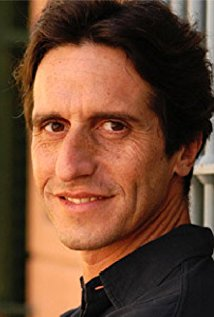
\includegraphics[width=100px]{peretti.jpg}
		\caption{Diego Peretti.}
		\label{peretti}
	\end{figure}
	
	\begin{figure}[H]
		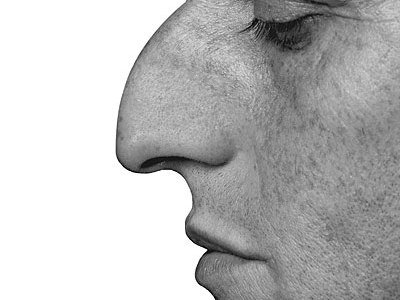
\includegraphics[width=150px]{nariz.jpg}
		\caption{La nariz de Diego Peretti.}
		\label{nariz}
	\end{figure}

\section{Complejidad}

	\subsection{Caracterizaci\'on del peor caso}
	El algoritmo, como vimos en la secci\'on 2, consiste en probar subconjuntos de agentes hasta encontrar la m\'axima cantidad de informantes que pueden agregarse a la soluci\'on sin que uno contradiga a otro. Como es requisito que el arreglo que representa a cada subconjunto est\'e ordenado, s\'olo vamos a probar con \textbf{una} representaci\'on de cada subconjunto, por lo que la cantidad de soluciones posibles se corresponde con la cantidad de subconjuntos distintos de $\{1,...,i\}$ (es decir, el \textit{cardinal del conjunto de partes} de $\{1,...,i\}$). Este n\'umero es $2^{i}$. La justificaci\'on la voy a escribir cuando aprenda a hacer footnotes.
	\\
	En el peor caso, el algoritmo tiene que probar \textbf{todos} los subconjuntos, o sea $2^{i}$ soluciones candidatas. Lo voy a justificar cuando efectivamente haya hecho el algoritmo.

	\subsection{C\'alculo de complejidad}
	La complejidad de este algoritmo, en el peor caso, es

	\begin{equation*}	
	T(n) \in \mathcal{O}(2^{i} \times i^{2} \times \log{i} \times a )
	\end{equation*}
	
	\paragraph{Justificaci\'on}
	Dado que el algoritmo debe probar 

\section{C\'odigo fuente}

\section{Experimentaci\'on}

\end{document}